\documentclass[10pt,twocolumn,letterpaper]{article}
\usepackage{cvpr}
\usepackage{times}
\usepackage{epsfig}
\usepackage{amsmath}
\usepackage{amssymb}
\usepackage{booktabs} % for much better looking tables
\usepackage{array} % for better arrays (eg matrices) in maths
\usepackage{paralist} % very flexible & customisable lists (eg. enumerate/itemize, etc.)
\usepackage{verbatim} % adds environment for commenting out blocks of text & for better verbatim
\usepackage{subfigure} % make it possible to include more than one captioned figure/table in a single float
\usepackage{graphicx}
\usepackage{multirow}
% Include other packages here, before hyperref.
% If you comment hyperref and then uncomment it, you should delete
% egpaper.aux before re-running latex.  (Or just hit 'q' on the first latex
% run, let it finish, and you should be clear).
%\usepackage[pagebackref=true,breaklinks=true,letterpaper=true,colorlinks,bookmarks=false]{hyperref}
\cvprfinalcopy % *** Uncomment this line for the final submission
\def\cvprPaperID{****} % *** Enter the CVPR Paper ID here
\def\httilde{\mbox{\tt\raisebox{-.5ex}{\symbol{126}}}}
% Pages are numbered in submission mode, and unnumbered in camera-ready
\ifcvprfinal\pagestyle{empty}\fi
\usepackage{url}

%use \x, \y, and \w for bold vector forms
%\newcommand{\x}{\bold{x}}
\DeclareMathOperator*{\argmax}{arg\,max}

\begin{document}
%%%%%%%%% TITLE
\title{
Project in CSE 250B\\
Assignment 4: Latent Dirichlet allocation models with Gibbs sampling}
\author{Andreas Landstad, Spencer Bliven, Jonas Hoelzler\\
Computer Science Department\\
University of California, San Diego\\
{\tt\small landstad.andreas@gmail.com, sbliven@ucsd.edu, jonas@hoelzler.de}
}% For a paper whose authors are all at the same institution,
% omit the following lines up until the closing ``}''.
% Additional authors and addresses can be added with ``\and'',
% just like the second author.
% To save space, use either the email address or home page, not both
%\and
%Second Author\\
%Institution2\\
%First line of institution2 address\\
%{\tt\small secondauthor@i2.org}
\maketitle
\thispagestyle{empty}
%%%%%%%%% ABSTRACT
\begin{abstract}
\end{abstract}
%%%%%%%%% BODY TEXT


\section{Introduction}
Latent Dirichlet allocation (LDA) is a generative process that can be used for modeling documents in order to find similarities between documents and within documents. This can be useful for clustering them, identifying categories within them or classifying them. In this paper we have used two training sets: 1. A set of documents with words and a set of topics to which the documents belong to. And 2. A set of  genomes with sequences of proteins and organisms to which these sequences belong to. The organisms can in this sense be thought of as topics and the proteins as words. By drawing topic distributions, $\phi_k$, according to the Dirichlet prior $\beta$ and then drawing a distribution over the words $\theta$ according to the Dirichlet prior $\alpha$, LDA is using these two drawn multinomials to draw a topic according to $\theta$ and and then a word according to $\phi_k$. In this way the parameter vectors for topics and words are learned. By using collapsed Gibb�s sampling as we have however, the the parameters $\phi$ and $\theta$ are not learned directly, but are instead hidden under parameters $z_i$ belonging to each word. Thus we are learning an estimated $p(z=j|z_j,w_i)$ for each word $i$ and topic $j$.

\section{Latent Dirichlet allocation}
For LDA a document is seen as a bag of words with no information about word order. We have a fixed vocabulary $V$ of all words that appear once in a document. Each document can then be represented as a vector of counts for each of these words. One word can appear within different topics and different documents can include words belonging to different topics. Because of this it is the different proportions of each of the topics for one document that is interesting for LDA. It is natural to represent the distribution of topics and words as multinomials, and this is why LDA uses a Dirichlet distribution. 

\begin{itemize}

\item bla
\item second

\end{itemize}

The Dirichlet distribution is the conjugate prior for multinomial distribution and LDA uses one Dirichlet distribution with parameter $\alpha$ as prior for the document distribution and one Dirichlet distribution with parameter $\beta$ for the per-topic word distribution. Then the generative process is as follows:
\begin{verbatim}
foreach topic $k$ draw a multinomial $\phi_k$ according to $\beta$
foreach document draw a multinomial $\theta$ according to $\alpha$
for each word $i$ in the document
draw a topic $z$ according to $\theta$
draw a word according to $\phi_z$
\end{verbatim}

\section{Gibb�s sampling}
As mentioned, by using collapsed Gibb�s sampling for learning, we don�t actually draw the multinomials $\theta$ and $\phi$ directly. Instead we have a hidden $z$ value for each appearance of each word in the training set. By drawing these $z$�s, Gibb�s sampling converges to a distribution of $z$-values for every word.
If $\bar{w}�$ is the entire corpora $\bar{w}$ with the word i removed, $\bar{w}�=w_i,\bar{w}�$ and $\bar{z}=z_i,\bar{z}�$ we compute:
$p(z_i|\bar{z}�,\bar{w})$=

\section{Document Dataset}
The document dataset has $K = 3$ topics. The LDA gibbs sampling was run over 344 iterations with $\alpha=1 and \beta = 0.01$. $\beta$ was selected according to \cite{griffiths}. $\alpha$ was selected small to guarantee fast convergence.  After 300 epochs it seemed to have converged to 96.75 \%. The euclidean distance between $\Theta$ and the true labels can be seen in Figure \ref{convergence}. The covergence against the final accuracy value of 96.75\% can be seen in Figure \ref{accuracy}. $\Phi$ shows the contribution in \% of every word to a topic. The ten words with the highest contribution are shown in Table ref{words}. One possible semantic interpretation of the topics could be Medicine, General Science and Aeronautical Engineering. In Figure \ref{simplex} one can see  s visualization of the documents based on the topics of the trained model, in 3D Euclidean space. One can see the underlying simplex lying in the 3D space.

\begin{figure*}[htbp] 
\centering
   \begin{minipage}{10 cm}
   \centering
    \includegraphics[width=10cm]{images/euclidean}
    \end{minipage}
  \caption{Convergence: Euclidean Distance to simplex of true labels}
  \label{convergence}
\end{figure*}

\begin{figure*}[htbp] 
\centering
   \begin{minipage}{10 cm}
   \centering
    \includegraphics[width=10cm]{images/accuracygrid}
    \end{minipage}
  \caption{Accuracy}
  \label{accuracy}
\end{figure*}


\begin{table}
    \begin{tabular}{|l|l|l|}
        \hline
        Topic 1 & Topic 2 & Topic 3 \\
    		\hline    
			  patients   &   system   &   boundary  \\
			  cases   &   problems   &   layer \\
			  ventricular   &   methods   &   wing  \\
			  fatty   &   research   &   mach  \\
			  left   &   scientific   &   supersonic  \\
			  nickel   &   development   &   ratio\\
			  time   &   retrieval   &   wings \\
			  acids   &   general   &   effects\\
			  aortic   &   part   &   velocity\\
			  free   &   language   &   shock\\
			  \hline
    \end{tabular}
\caption{The words with highest overall $\Phi$ values of the three categories. One possible interpretation of the topics could be Medicine, General Science and Aeronautical Engineering}
\label{words}
\end{table}
%Values
 %   0.0113    0.0083    0.0111
 %   0.0073    0.0069    0.0089
 %   0.0073    0.0067    0.0084
 %   0.0066    0.0065    0.0073
 %   0.0064    0.0063    0.0071
 %   0.0064    0.0059    0.0060
 %   0.0062    0.0058    0.0058
 %   0.0060    0.0055    0.0058
 %   0.0049    0.0049    0.0058
 %   0.0047    0.0048    0.0056


%
%\begin{figure*}[htbp] 
%\centering
%   \begin{minipage}{10 cm}
%   \centering
%    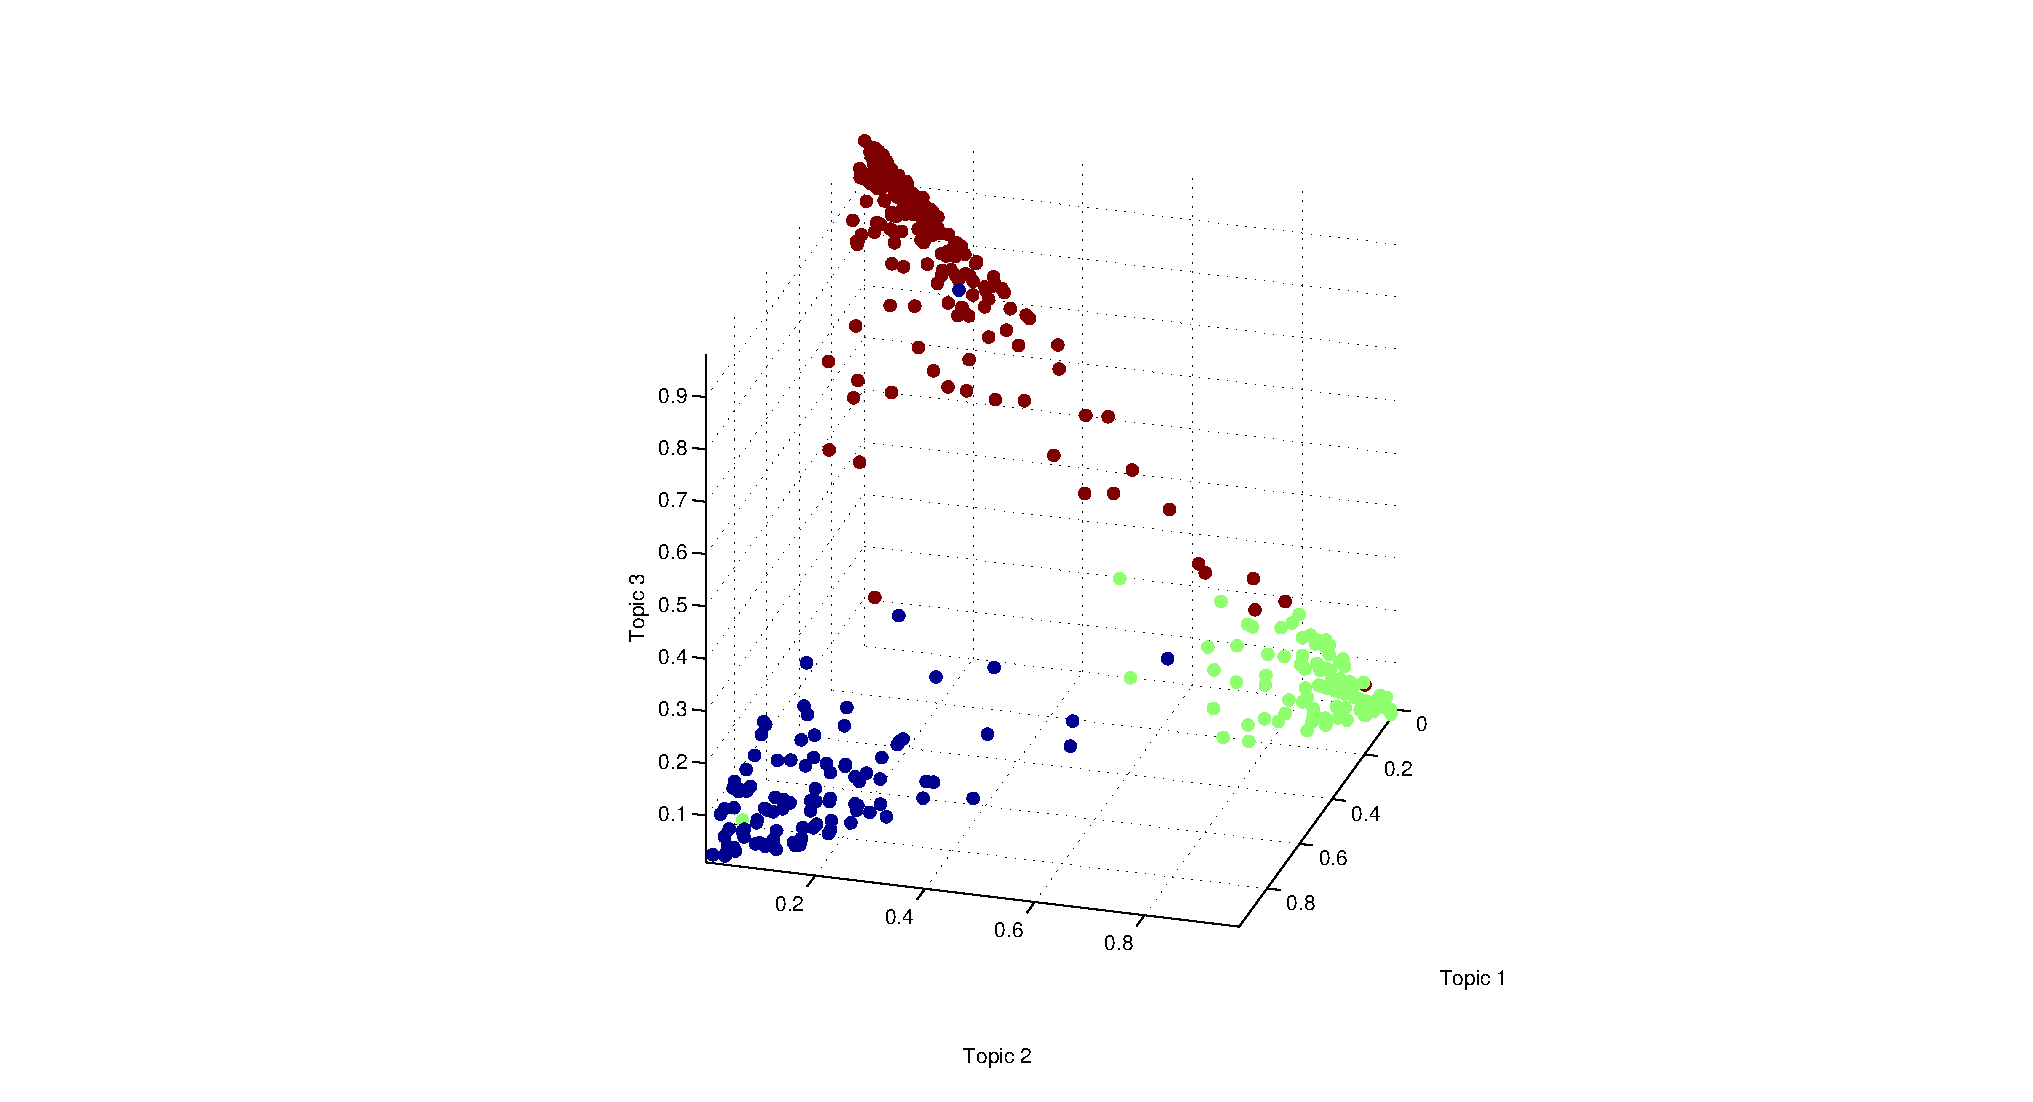
\includegraphics[width=10cm]{images/simplex}
%    \end{minipage}
%  \caption{Simplex of document dataset. The colors show the truelabels. There are 13 wrong classifications. Most classifications are wrong between topic 1 and topic 3, which are not very similar to topic 2.}
%  \label{Labelname}
%\end{figure*}


\section{Genome Dataset}

Although LDA is couched in terms of words and documents, the LDA model can be extended to any type of information which is expressed as a sequence over some abstract alphabet. To demonstrate this, we encode genomes as sequences of proteins, and use LDA to classify organisms.

The genome of an organism can be thought of as a long sequence of genes. Since closely related genes tend to be functionally similar, genes can be classified into families. One organism may contain several copies of genes from the same family, and a broad range of species may have genes belonging to the same family. Thus, the concept of a �bag of words� representation for text documents can be extended to a �bag of gene families� representation of single genomes. Such a representation was generated for a wide range of genomes and is refered to as the \begin{em}genome dataset\end{em}. 

\subsection{Construction of the Genome Dataset}

%added
%The UniProt Consortium
%Ongoing and future developments at the Universal Protein Resource
%Nucleic Acids Res. 39: D214-D219 (2011).

%add
%Jain E., Bairoch A., Duvaud S., Phan I., Redaschi N., Suzek B.E., Martin M.J., McGarvey P., Gasteiger E.
%Infrastructure for the life sciences: design and implementation of the UniProt website
%BMC Bioinformatics 2009, 10:136.

%           The Pfam protein families database: R.D. Finn, J. Mistry, J. Tate, P. Coggill, A. Heger, J.E. Pollington, O.L. Gavin, P. Gunesekaran, G. Ceric, K. Forslund, L. Holm, E.L. Sonnhammer, S.R. Eddy, A. Bateman Nucleic Acids Research (2010)  Database Issue 38:D211-222


Initially, 1207 species were selected for analysis based on their annotation in UniProt (release 2011\textunderscore 03) \cite{uniprot} as being �complete� and �reviewed and annotated�\footnote{For more information about compete genomes, see \url{http://www.uniprot.org/faq/15}}. All Swiss-Prot entries \cite{swissprot} for each species were subsequently downloaded and used to define the genome of each species. Note that the automatically annotated TrEMBL database was not used for performance reasons, although automatic curations would have significantly increased the number of genes considered for some organisms. In total, 525,997 unique genes were considered.

The Pfam database was used to cluster genes into families. There are 11,912 families in the Pfam database (Pfam A, version 24, Oct 2009), which clusters UniProt proteins into families according to a set of profile hidden Markov models.  429,383 unique matches of protein families were mapped to the genomes, with a duplication within genomes giving a total of 685,267 proteins.

After mapping pfams onto genomes, 141 genomes were discarded due to zero coverage by Pfam. These genomes were likely sequenced after the last update of Pfam in late 2009. Additionally, 3560 Pfam families were discarded because they did not map to any of the species concidered. After this filtering, the genome dataset consisted of 1066 genomes over a vocabulary of        8352 protein families.

\section{Discussion}

\subsection{Distribution of Genome Dataset}

Out of the 1066 genomes concidered in the genome dataset, 12\% came from Eukaryota,    7\% from Archaea, and    81\% from Bacteria. This distribution reflects the large amount of bacteria which have been recently sequenced. However, it should be noted that many of the bacteria included are closely related. For instance, 35 strains of \begin{em}E. coli\end{em} have been completely sequenced, do to the importance of this bacteria as a model organism and the relative inexpensiveness of resequencing a bacterial genome.
%Thus, while the majority of genomes come from Bacteria, documents tend to be more similar.

\begin{figure}[htbp]
 \centering
 \begin{minipage}[b]{5 cm}
    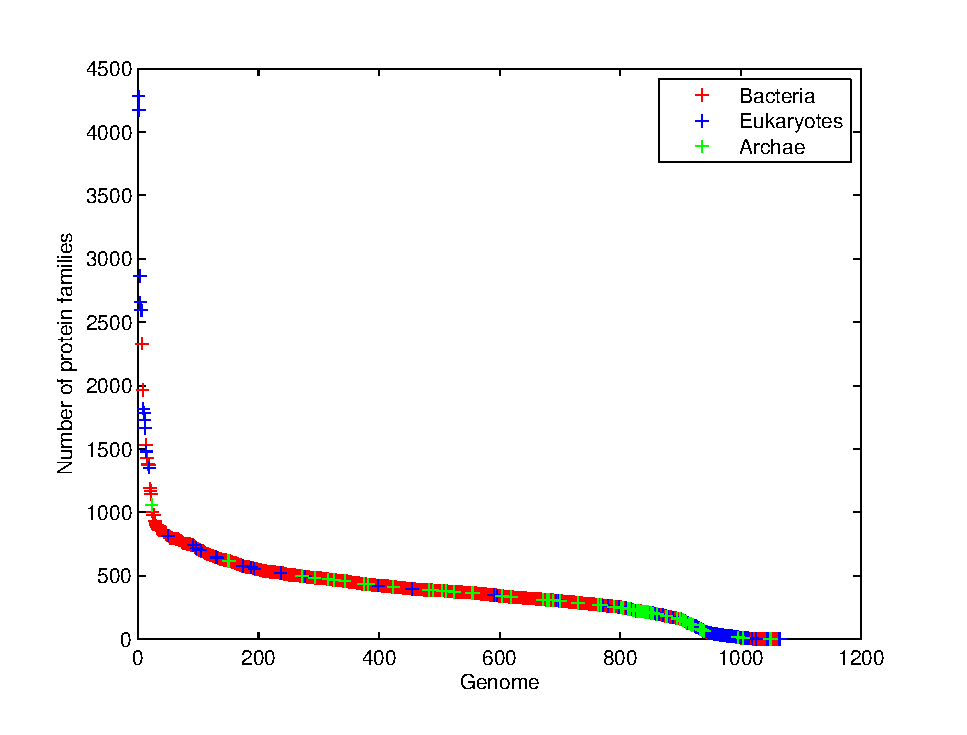
\includegraphics[width=10cm]{images/proteinsPerGenome}
   \caption{proteins}
   \label{Labelname 1}
 \end{minipage}
 \begin{minipage}[b]{5 cm}
    \includegraphics[width=10cm]{images/genomesPerProtein}
   \caption{genomes}
   \label{Labelname 2}
 \end{minipage}
\end{figure}


\nocite{blei02,elkan11,bishop06}




{\small
\bibliographystyle{ieee}
\bibliography{egbib}
}
\end{document}
